\documentclass[autocontact]{gaceta}
\usepackage[utf8]{inputenc}

%---------------------
%-----librerias para los grafos
\usepackage{tikz}
\usetikzlibrary{positioning}
\definecolor {processblue}{cmyk}{0.96,0,0,0}
%---------------------
% Esto ya lo carga el estilo de La Gaceta:
\usepackage{amsmath, amsthm, amssymb}
%\usepackage{url} % <-- Para p\'aginas web o similar: \url{...}
\usepackage{graphicx}
%---------------------

%---------------------
% Carga esto para gr\'aficos si lo necesitas:
% \usepackage{wrapfig}
%---------------------

%---------------------
% <<< ESTO SE AJUSTAR\'A AL EDITAR CADA N\'UMERO DE LA GACETA >>>
\setcounter{page}{1} 
\journame{UAdeC-FCFM}
\yearofpublication{2018}
\volume{1}
\issuenumber{0}
%---------------------

%---------------------
% Deja esto as\'{\i}:
\belongstopart{Art\'{\i}culos} 


%---------------------
\title{Universidad Autónoma de Coahuila \\ Facultad de Ciencias Físico Matemáticas
\\ Investigación de operaciones \\ Teoría de Grafos \\ Tarea 2 \\ Alibeit Kakes}
\author{Jesús López Zavala} % o \author{Un Autor y Otro Autor}, etc.
% Opcional:
\shorttitle{Ejemplo de c\'omo escribir un art\'{\i}culo para La Gaceta}
%---------------------

%---------------------
\contact{Un autor, Dpto. de Matem\'aticas, Universidad de \dots}
{autor@uni.es}{http://www.uni.es/personales/autor.html}
%% SINTAXIS (\'usense tantos de estos como autores haya):
%\contact{nombre y direcci\'on autor 1}{email autor 1}{p\'agina web autor 1}
%\contact{nombre y direcci\'on autor 2}{email autor 2}{p\'agina web autor 2}
% (IMPORTANTE: se puede dejar vac\'{\i}o lo que se quiera)
%---------------------

%---------------------------
\begin{document}
\maketitle
%---------------------





%%---------------------------Problema1----------------------------------
%-----------------------------------------------------------------------
\section{Problema 1}
    Encontrar el camino de longitud máxima que une los nodos $x_{1}$ y $x_{6}$.
    
    \tikzstyle{camino}=[bottom color = processblue!20, draw,processblue, text = red]
    \tikzstyle{place}=[circle,draw=blue!50,fill=blue!20,thick]
    \tikzstyle{transition}=[rectangle,draw=black!50,fill=black!20,thick]
    \tikzstyle{every label}= [blue]
    
    \begin{figure}[h]

    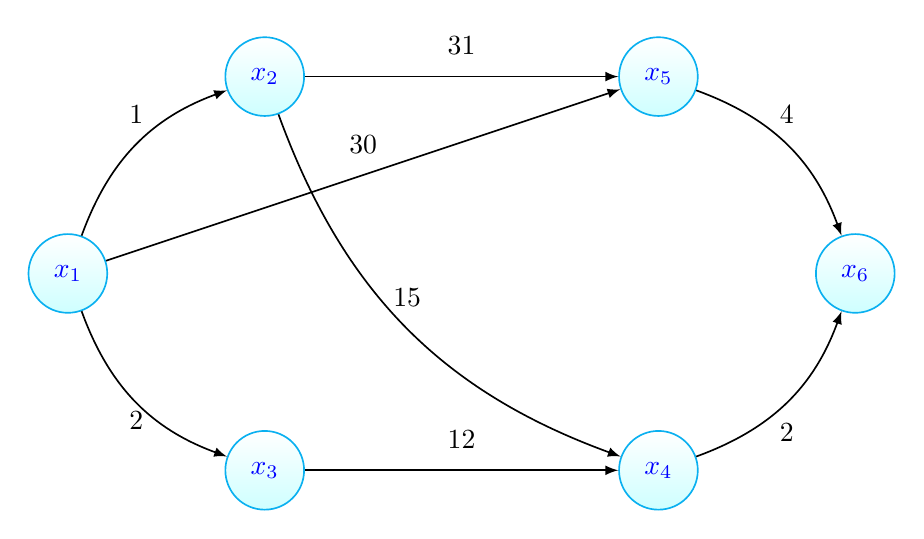
\begin{tikzpicture}[-latex, auto, node distance =4 cm and 5cm, on grid , semithick, scale = 1.0,
                state/.style ={ circle ,top color =white , bottom color = processblue!20 ,
                draw,processblue , text=blue , minimum width =1 cm, scale = 1.0}]
            
            %\node [estilo del nodo] (nombre del nodo) [posicion relativa]/at (posicion,absoluta) {};
            \node[state] (n1) at (-5, 0) {$x_1$};
            \node[state] (n2) at (-2.5, 2.5) {$x_2$};
            \node[state] (n3) at (-2.5, -2.5) {$x_3$};
            \node[state] (n4) at (2.5, -2.5) {$x_4$};
            \node[state] (n5) at (2.5, 2.5) {$x_5$};
            \node[state] (n6) at (5, 0) {$x_6$};
            

            \path (n1) edge [bend right = -25] node[above = 0.15 cm] {$1$} (n2);
            \path (n1) edge [bend right = 25] node[below = 0.0 cm] {$2$} (n3);
            \path (n2) edge  node[above = 0.15 cm] {$31$} (n5);
            \path (n3) edge  node[above = 0.15 cm] {$12$} (n4);
            \path (n5) edge  [bend right = -25] node[above = 0.15 cm] {$4$} (n6);
            \path (n4) edge  [bend right = 25] node[below = 0.15 cm] {$2$} (n6);
            \path (n1) edge  node[above = 0.15 cm] {$30$} (n5);
            \path (n2) edge  [bend right = 25] node[above = 0.15 cm] {$15$} (n4);
            %si queremos un loop
            %\path (A) edge [loop left] node[left] {$1/4$} (A);
    \end{tikzpicture}
    
    \caption{}
\end{figure}

    Para resolverlo hay que aplicar el algoritmo de Ford, a continuación se muestran las
    marcas sobre cada nodo:

    
    \begin{tikzpicture}[-latex, auto, node distance =4 cm and 5cm, on grid , semithick, scale = 1.0,
            state/.style ={ circle ,top color =white , bottom color = processblue!20 ,
            draw,processblue , text=blue , minimum width =1 cm, scale = 1.0}]
        
        %\node [estilo del nodo] (nombre del nodo) [posicion relativa]/at (posicion,absoluta) {};
        \node[state] (n1) at (-5, 0) [label=left:$ (-{,}0) $] {$x_1$};
        \node[state] (n2) at (-2.5, 2.5) [label = above: $ (x_1 {,} 1) $] {$x_2$};
        \node[state] (n3) at (-2.5, -2.5) [label = above: $ (x_1 {,} 2) $] {$x_3$};
        \node[state] (n4) at (2.5, -2.5) [label = above: $ (x_2 {,} 16) $] {$x_4$};
        \node[state] (n5) at (2.5, 2.5) [label = above: $ (x_2 {,} 32) $] {$x_5$};
        \node[state] (n6) at (5, 0) [label = right: $ (x_5 {,} 36) $] {$x_6$};
        

        \path (n1)[camino] edge [bend right = -25] node[above = 0.15 cm] {$1$} (n2);
        \path (n1) edge [bend right = 25] node[below = 0.0 cm] {$2$} (n3);
        \path (n2)[camino] edge  node[above = 0.15 cm] {$31$} (n5);
        \path (n3) edge  node[above = 0.15 cm] {$12$} (n4);
        \path (n5)[camino] edge  [bend right = -25] node[above = 0.15 cm] {$4$} (n6);
        \path (n4) edge  [bend right = 25] node[below = 0.15 cm] {$2$} (n6);
        \path (n1) edge  node[above = 0.15 cm] {$30$} (n5);
        \path (n2) edge  [bend right = 25] node[above = 0.15 cm] {$15$} (n4);
        %si queremos un loop
        %\path (A) edge [loop left] node[left] {$1/4$} (A);
    \end{tikzpicture}

    Para encontrar el camino óptimo realizamos la siguiente operación:
    $$ e(j) - e(i) = c(ij)$$
    y si esta ecuación se cumple entonces nos quedamos con el arco entre ambas marcas.
    Este análisis conduce al siguiente conjunto de arcos que conforman el camino de longitud máxima:
    $$ U = \{ (x_1, x_2), (x_2, x_5), (x_5, x_6) \} $$






%%---------------------------Problema2----------------------------------
%-----------------------------------------------------------------------

\section{}
    ¿Podemos conocer la longitud del camino extremal sin conocer explícitamente los arcos que la 
    componen?. ¿Se pueden marcar más de una vez los vértices? \\
    \\Para conocer la longitud del camino extremal es necesario conocer explícitamente
        la relacion que existe entre los vértices (arcos), así como el valor que cada uno de los arcos tiene
        asignado. Si marcamos más de una vez los vértices, entonces habrá ambiguedad y el algoritmo con el que
        se esté trabajando, para nuestro caso el algoritmo de Ford, no estará cumpliendo con el objetivo de 
        encontrar un camino extremal.





%%---------------------------Problema3----------------------------------
%-----------------------------------------------------------------------
\section{}
    Formule el algoritmo de Ford para hallar caminos mínimos.\\
    \\Supongamos que se quiere encontrar el camino mínimo entre los vértices $s$ y $t$ de algún grafo dado,
        para hacerlo formularemos el algoritmo de Ford como sigue:
        \begin{center}
            \begin{enumerate}
                \item Marcar el vértice $s$ con la marca $(-, 0)$.
                \item Marcar el vértice $j$ con la marca $(i, e(j))$, con $$ e(j) = min \{e(i) + c(ij)\}$$.
                \item Aplicar el paso anterior hasta llegar al vértice $t$.
                \item Para encontrar el camino mínimo se hace un recorrido desde el vértice $t$ hasta el 
                        vértice $s$ buscando los arcos tales que cumplan: $$e(j) - e(i) = c(i,j),$$ \\de 
                        forma que el conjunto de arcos encontrados es el camino mínimo.
            \end{enumerate}
        \end{center}





%%---------------------------Problema4----------------------------------
%-----------------------------------------------------------------------
\section{Problema 4}
    En el grafo del ejercicio 1, halle el camino de longitud mínima.\\
    \\A continuación se muestran las marcas obtenidas al aplicar el algoritmo de Ford 
    descrito anteriormente:
    
       
    \begin{tikzpicture}[-latex, auto, node distance =4 cm and 5cm, on grid , semithick, scale = 1.0,
        state/.style ={ circle ,top color =white , bottom color = processblue!20 ,
        draw,processblue , text=blue , minimum width =1 cm, scale = 1.0}]
    
        %\node [estilo del nodo] (nombre del nodo) [posicion relativa]/at (posicion,absoluta) {};
        \node[state] (n1) at (-5, 0) [label=left:$ (-{,}0) $] {$x_1$};
        \node[state] (n2) at (-2.5, 2.5) [label = above: $ (x_1 {,} 1) $] {$x_2$};
        \node[state] (n3) at (-2.5, -2.5) [label = above: $ (x_1 {,} 2) $] {$x_3$};
        \node[state] (n4) at (2.5, -2.5) [label = above: $ (x_3 {,} 14) $] {$x_4$};
        \node[state] (n5) at (2.5, 2.5) [label = above: $ (x_1 {,} 30) $] {$x_5$};
        \node[state] (n6) at (5, 0) [label = right: $ (x_4 {,} 16) $] {$x_6$};
        

        \path (n1) edge [bend right = -25] node[above = 0.15 cm] {$1$} (n2);
        \path (n1)[camino] edge [bend right = 25] node[below = 0.0 cm] {$2$} (n3);
        \path (n2) edge  node[above = 0.15 cm] {$31$} (n5);
        \path (n3)[camino] edge  node[above = 0.15 cm] {$12$} (n4);
        \path (n5) edge  [bend right = -25] node[above = 0.15 cm] {$4$} (n6);
        \path (n4)[camino] edge  [bend right = 25] node[below = 0.15 cm] {$2$} (n6);
        \path (n1) edge  node[above = 0.15 cm] {$30$} (n5);
        \path (n2) edge  [bend right = 25] node[above = 0.15 cm] {$15$} (n4);
        %si queremos un loop
        %\path (A) edge [loop left] node[left] {$1/4$} (A);
    \end{tikzpicture}


    Aplicando el paso $4$ descrito en el problema anterior obtenemos el siguente conjunto de arcos:
    $$ U = \{ (x_1, x_3), (x_3, x_4), (x_4, x_6)\}, $$
    siendo éste el camino de longitud mínima.



%%---------------------------Problema5----------------------------------
%-----------------------------------------------------------------------
\section{Problema 5}
En el grafo siguiente halle:
    \begin{enumerate}
        \item Encontrar el camino de longitud máxima que une los nodos $\alpha$ y $\beta$.
        \item Encontrar el camino de longitud mínima que une los nodos $\alpha$ y $\beta$.
        \item El recorrido que acumule la menor cantidad de arcos, de $\alpha$ a $\beta$.
    \end{enumerate}

    
    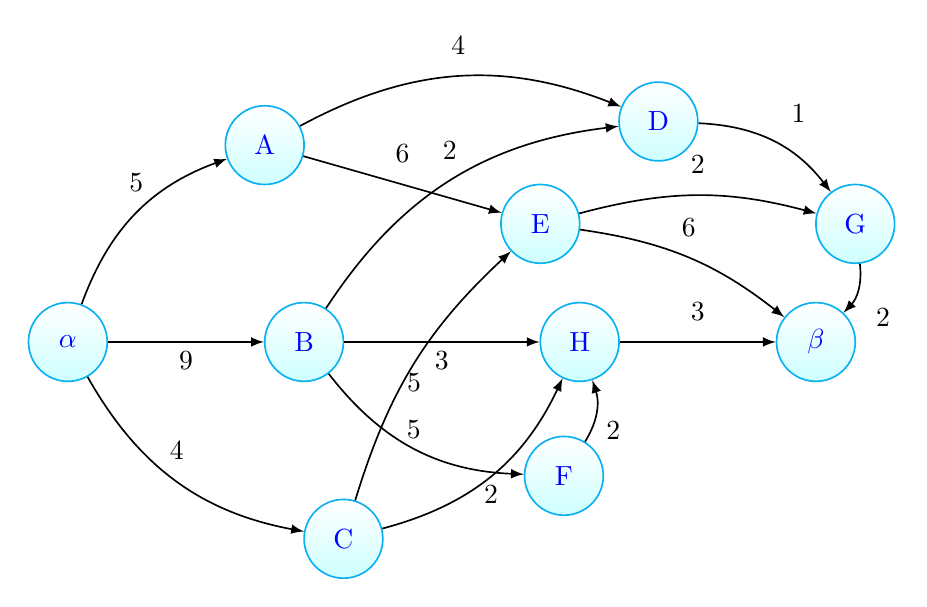
\begin{tikzpicture}[-latex, auto, node distance =4 cm and 5cm, on grid , semithick, scale = 1.0,
            state/.style ={ circle ,top color =white , bottom color = processblue!20 ,
            draw,processblue , text=blue , minimum width =1 cm, scale = 1.0}]
        
        %\node [estilo del nodo] (nombre del nodo) [posicion relativa]/at (posicion,absoluta) {};
        \node[state] (a) at (-5, 0) {$\alpha$};
        \node[state] (A) at (-2.5, 2.5) {A};
        \node[state] (B) at (-2.0, 0) {B};
        \node[state] (C) at (-1.5, -2.5) {C};
        \node[state] (E) at (1.0, 1.5) {E};
        \node[state] (H) at (1.5, 0) {H};
        \node[state] (F) at (1.3, -1.7) {F};
        \node[state] (D) at (2.5, 2.8) {D};
        \node[state] (b) at (4.5, 0) {$\beta$};
        \node[state] (G) at (5.0, 1.5) {G};
        

        \path (a) edge [bend right = -25] node[above = 0.15 cm] {$5$} (A);
        \path (a) edge node[below = 0.0 cm] {$9$} (B);
        \path (a) edge [bend right = 25] node[above = 0.15 cm] {$4$} (C);
        \path (A) edge [bend right = -25] node[above = 0.15 cm] {$4$} (D);
        \path (A) edge node[above = 0.15 cm] {$6$} (E);
        \path (B) edge  [bend right = -25] node[above = 0.15 cm] {$2$} (D);
        \path (B) edge  node[below = 0.0 cm] {$3$} (H);
        \path (B) edge  [bend right = 25] node[above = 0.0 cm] {$5$} (F);
        \path (C) edge [bend right = -15] node[below = 0.0 cm] {$5$} (E);
        \path (C) edge [bend right = 25] node[below = 0.0 cm] {$2$} (H);
        \path (F) edge [bend right = 25] node[below right = 0.0 cm] {$2$} (H);
        \path (H) edge node[above = 0.15 cm] {$3$} (b);
        \path (G) edge [bend right = -25] node[below right = 0.15 cm] {$2$} (b);
        \path (D) edge [bend right = -25] node[above right = 0.15 cm] {$1$} (G);
        \path (E) edge [bend right = -15] node[above = 0.15 cm] {$2$} (G);
        \path (E) edge [bend right = -15] node[above = 0.15 cm] {$6$} (b);
        
        %si queremos un loop
        %\path (A) edge [loop left] node[left] {$1/4$} (A);
    \end{tikzpicture}

    1. Aplicando el algoritmo de Ford se obtiene que el conjunto:
    $$ U = \{ (\alpha, B), (B, F), (F, H), (H, \beta) \}, $$
    es el camino de longitud máxima. A continuación se muestra en la figura a este conjunto de arcos 
    coloreados en tono azul:

        \begin{tikzpicture}[-latex, auto, node distance =4 cm and 5cm, on grid , semithick, scale = 1.0,
        state/.style ={ circle ,top color =white , bottom color = processblue!20 ,
        draw,processblue , text=blue , minimum width =1 cm, scale = 1.0}]
    
    %\node [estilo del nodo] (nombre del nodo) [posicion relativa]/at (posicion,absoluta) {};
    \node[state] (a) at (-5, 0) [label = left: $ (- {,} 0) $] {$\alpha$};
    \node[state] (A) at (-2.5, 2.5) [label = above: $ (\alpha {,} 5) $] {A};
    \node[state] (B) at (-2.0, 0) [label = above left: $ (\alpha {,} 9) $] {B};
    \node[state] (C) at (-1.5, -2.5) [label = above left: $ (\alpha {,} 4) $] {C};
    \node[state] (E) at (1.0, 1.5) [label = above: $ (A {,} 11) $] {E};
    \node[state] (H) at (1.5, 0) [label = above: $ (F {,} 16) $] {H};
    \node[state] (F) at (1.3, -1.7) [label = below: $ (B {,} 14) $] {F};
    \node[state] (D) at (2.5, 2.8) [label = above: $ (B {,} 11) $] {D};
    \node[state] (b) at (4.5, 0) [label = above: $ (H {,} 19) $] {$\beta$};
    \node[state] (G) at (5.0, 1.5) [label = above: $ (E {,} 13) $] {G};
    

    \path (a) edge [bend right = -25] node[above = 0.15 cm] {$5$} (A);
    \path (a)[camino] edge node[below = 0.0 cm] {$9$} (B);
    \path (a) edge [bend right = 25] node[above = 0.15 cm] {$4$} (C);
    \path (A) edge [bend right = -25] node[above = 0.15 cm] {$4$} (D);
    \path (A) edge node[above = 0.15 cm] {$6$} (E);
    \path (B) edge  [bend right = -25] node[above = 0.15 cm] {$2$} (D);
    \path (B) edge  node[below = 0.0 cm] {$3$} (H);
    \path (B)[camino] edge  [bend right = 25] node[above = 0.0 cm] {$5$} (F);
    \path (C) edge [bend right = -15] node[below = 0.0 cm] {$5$} (E);
    \path (C) edge [bend right = 25] node[below = 0.0 cm] {$2$} (H);
    \path (F)[camino] edge [bend right = 25] node[below right = 0.0 cm] {$2$} (H);
    \path (H)[camino] edge node[above = 0.15 cm] {$3$} (b);
    \path (G) edge [bend right = -25] node[below right = 0.15 cm] {$2$} (b);
    \path (D) edge [bend right = -25] node[above right = 0.15 cm] {$1$} (G);
    \path (E) edge [bend right = -15] node[above = 0.15 cm] {$2$} (G);
    \path (E) edge [bend right = -15] node[above = 0.15 cm] {$6$} (b);


    %si queremos un loop
    %\path (A) edge [loop left] node[left] {$1/4$} (A);
\end{tikzpicture}


    2. El algoritmo de Ford para encontrar caminos mínimos conduce a que el siguiente conjunto:
    $$ U = \{ (\alpha, C), (C, H), (H, \beta) \}, $$
    es el camino de longitud mínima.\\ A continuación se muestra la figura con las marcas resultantes 
    en cada vértice, así como los arcos que conforman 
    al conjunto $U$. Dichos arcos estan coloreados en azul y sus respectivas longitudes se muestran en color
    rojo:

        \begin{tikzpicture}[-latex, auto, node distance =4 cm and 5cm, on grid , semithick, scale = 1.0,
        state/.style ={ circle ,top color =white , bottom color = processblue!20 ,
        draw,processblue , text=blue , minimum width =1 cm, scale = 1.0}]
    
    %\node [estilo del nodo] (nombre del nodo) [posicion relativa]/at (posicion,absoluta) {};
    \node[state] (a) at (-5, 0) [label = left: $ (- {,} 0) $] {$\alpha$};
    \node[state] (A) at (-2.5, 2.5) [label = above: $ (\alpha {,} 5) $] {A};
    \node[state] (B) at (-2.0, 0) [label = above left: $ (\alpha {,} 9) $] {B};
    \node[state] (C) at (-1.5, -2.5) [label = above left: $ (\alpha {,} 4) $] {C};
    \node[state] (E) at (1.0, 1.5) [label = above: $ (C {,} 9) $] {E};
    \node[state] (H) at (1.5, 0) [label = above: $ (C {,} 6) $] {H};
    \node[state] (F) at (1.3, -1.7) [label = below: $ (B {,} 14) $] {F};
    \node[state] (D) at (2.5, 2.8) [label = above: $ (A {,} 9) $] {D};
    \node[state] (b) at (4.5, 0) [label = above: $ (H {,} 9) $] {$\beta$};
    \node[state] (G) at (5.0, 1.5) [label = above: $ (D {,} 10) $] {G};
    

    \path (a) edge [bend right = -25] node[above = 0.15 cm] {$5$} (A);
    \path (a) edge node[below = 0.0 cm] {$9$} (B);
    \path (a)[camino] edge [bend right = 25] node[above = 0.15 cm] {$4$} (C);
    \path (A) edge [bend right = -25] node[above = 0.15 cm] {$4$} (D);
    \path (A) edge node[above = 0.15 cm] {$6$} (E);
    \path (B) edge  [bend right = -25] node[above = 0.15 cm] {$2$} (D);
    \path (B) edge  node[below = 0.0 cm] {$3$} (H);
    \path (B) edge  [bend right = 25] node[above = 0.0 cm] {$5$} (F);
    \path (C) edge [bend right = -15] node[below = 0.0 cm] {$5$} (E);
    \path (C)[camino] edge [bend right = 25] node[below = 0.0 cm] {$2$} (H);
    \path (F) edge [bend right = 25] node[below right = 0.0 cm] {$2$} (H);
    \path (H)[camino] edge node[above = 0.15 cm] {$3$} (b);
    \path (G) edge [bend right = -25] node[below right = 0.15 cm] {$2$} (b);
    \path (D) edge [bend right = -25] node[above right = 0.15 cm] {$1$} (G);
    \path (E) edge [bend right = -15] node[above = 0.15 cm] {$2$} (G);
    \path (E) edge [bend right = -15] node[above = 0.15 cm] {$6$} (b);


    %si queremos un loop
    %\path (A) edge [loop left] node[left] {$1/4$} (A);
\end{tikzpicture}

    3. Para responder a esta pregunta, sustituiremos los valores predeterminados en cada 
    arco por el valor de 1, luego aplicaremos el algoritmo de Ford para encontrar así 
    todos los posibles conjuntos con el menor número de arcos.
    Luego de aplicar el algoritmo, el grafo reslultante se muestra a continuación:


    \begin{figure}[h]


\begin{tikzpicture}[-latex, auto, node distance =4 cm and 5cm, on grid , semithick, scale = 1.0,
        state/.style ={ circle ,top color =white , bottom color = processblue!20 ,
        draw,processblue , text=blue , minimum width =1 cm, scale = 1.0}]
    
        %\node [estilo del nodo] (nombre del nodo) [posicion relativa]/at (posicion,absoluta) {};
        \node[state] (a) at (-5, 0) [label = left: $ (- {,} 0) $] {$\alpha$};
        \node[state] (A) at (-2.5, 2.5) [label = above: $ (\alpha {,} 1) $] {A};
        \node[state] (B) at (-2.0, 0) [label = above left: $ (\alpha {,} 1) $] {B};
        \node[state] (C) at (-1.5, -2.5) [label = above left: $ (\alpha {,} 1) $] {C};
        \node[state] (E) at (1.0, 1.5) [label = above: $ (A {,} 2) $] [label = above right: $ (C {,} 2) $] {E};
        \node[state] (H) at (1.5, 0) [label = above: $ (F {,} 3) $] {H};
        \node[state] (F) at (1.3, -1.7) [label = below: $ (B {,} 2) $] {F};
        \node[state] (D) at (2.5, 2.8) [label = above: $ (A {,} 2) $] [label = above right: $ (B {,} 2) $] {D};
        \node[state] (b) at (4.5, 0) [label = below left: $ (H {,} 4) $] [label = below: $ (G {,} 4) $] {$\beta$};
        \node[state] (G) at (5.0, 1.5) [label = above: $ (D {,} 3) $] [label = above right: $ (E {,} 3) $] {G};
        

        \path (a) edge [bend right = -25] node[above = 0.15 cm] {$1$} (A);
        \path (a)[camino] edge node[below = 0.0 cm] {$1$} (B);
        \path (a) edge [bend right = 25] node[above = 0.15 cm] {$1$} (C);
        \path (A) edge [bend right = -25] node[above = 0.15 cm] {$1$} (D);
        \path (A) edge node[above = 0.15 cm] {$1$} (E);
        \path (B) edge  [bend right = -25] node[above = 0.15 cm] {$1$} (D);
        \path (B)[camino] edge  node[below = 0.0 cm] {$1$} (H);
        \path (B) edge  [bend right = 25] node[above = 0.0 cm] {$1$} (F);
        \path (C) edge [bend right = -15] node[below = 0.0 cm] {$1$} (E);
        \path (C) edge [bend right = 25] node[below = 0.0 cm] {$1$} (H);
        \path (F) edge [bend right = 25] node[below right = 0.0 cm] {$1$} (H);
        \path (H)[camino] edge node[above = 0.15 cm] {$1$} (b);
        \path (G) edge [bend right = -25] node[below right = 0.15 cm] {$1$} (b);
        \path (D) edge [bend right = -25] node[above right = 0.15 cm] {$1$} (G);
        \path (E) edge [bend right = -15] node[above = 0.15 cm] {$1$} (G);
        \path (E) edge [bend right = -15] node[above = 0.15 cm] {$1$} (b);


        %si queremos un loop
        %\path (A) edge [loop left] node[left] {$1/4$} (A);
    \end{tikzpicture}
    
    \caption{En azul uno de los caminos con menor cantidad de arcos.}
\end{figure}


%%---------------------------Otros problemas----------------------------------
%-----------------------------------------------------------------------
\section{Problema que resolvimos en clase}
   \begin{figure}[h]

 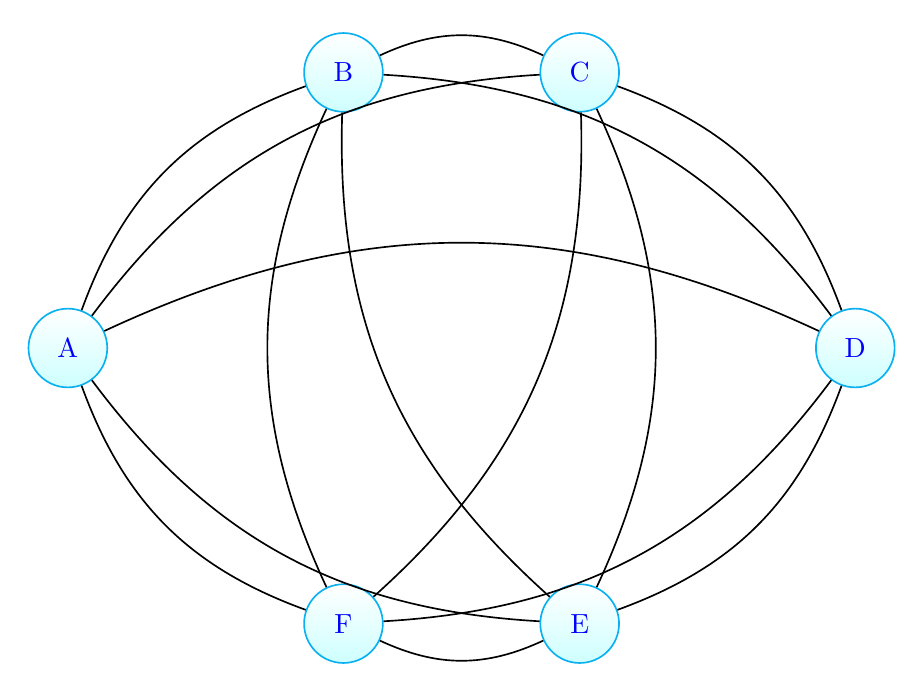
\begin{tikzpicture}[auto, node distance =4 cm and 5cm, on grid , semithick, scale = 1.0,
            state/.style ={ circle ,top color =white , bottom color = processblue!20 ,
            draw,processblue , text=blue , minimum width =1 cm}]
        
        %\node [estilo del nodo] (nombre del nodo) [posicion relativa]/at (posicion,absoluta) {};
        
        \node[state] (A) at (-5, 0) {A};
        \node[state] (B) at (-1.5, 3.5) {B};
        \node[state] (C) at (1.5, 3.5) {C};
        \node[state] (D) at (5, 0) {D};
        \node[state] (E) at (1.5, -3.5) {E};
        \node[state] (F) at (-1.5, -3.5) {F};
        
        \path (A) edge [bend right = -25] (B);
        \path (A) edge [bend right = -25] (C);
        \path (A) edge [bend right = -25] (D);
        \path (A) edge [bend right = 25] (E);
        \path (A) edge [bend right = 25] (F);
        
        \path (B) edge [bend right = -25] (C);
        \path (B) edge [bend right = -25] (D);
        \path (B) edge [bend right = 25] (E);
        \path (B) edge [bend right = 25] (F);

        \path (C) edge [bend right = -25] (D);
        \path (C) edge [bend right = -25] (E);
        \path (C) edge [bend right = -25] (F);

        \path (D) edge [bend right = -25] (E);
        \path (D) edge [bend right = -25] (F);

        \path (E) edge [bend right = -25] (F);




        %si queremos un loop
        %\path (A) edge [loop left] node[left] {$1/4$} (A);
        
    \end{tikzpicture}
     \caption{}
\end{figure}  




%---------------------------
\end{document}
%---------------------------

